\section{Développement du noyau formel : conditions initiales, géométrie et raffinement}
\label{sec:extension}

Le support de quatre-vingt-une positions ne coïncide pas avec le domaine des conditions initiales de la dynamique. Une condition initiale doit également indiquer une orientation ; les feuillets additif et multiplicatif disposent en outre de curseurs indépendants. Cette distinction permet de reconstruire exhaustivement l’émission sans sélectionner au préalable une région numérique.

\subsection{Les états initiaux et la récurrence d’émission}

Pour l’énumération, nous utilisons les indices \(I_9=\{0,\ldots,8\}\), reliés aux étiquettes positives par \(i\mapsto i+1\). Soit
\[
 \mathcal S=I_9^2\times\{N,E,S,O\},\qquad
 \Omega_{\rm seed}=\mathcal S_+\times\mathcal S_\times.
\]
Chaque condition initiale \(\omega=(s_+,s_\times)\) détermine deux positions et deux directions. Le domaine comprend tous les couples ordonnés, de sorte que
\begin{equation}
 |\mathcal S|=324,\qquad |\Omega_{\rm seed}|=324^2=104\,976.
 \label{eq:semillas}
\end{equation}
Le paramétrage précédent est déjà une énumération interne : chacune des
\(81\) paires de positions apparaît avec les quatre directions, et le produit
cartésien conserve les \(324^2\) combinaisons des deux curseurs. Les lignes
d’un tableau d’émissions sont des fibres de ce domaine de conditions initiales ;
aucun catalogue extérieur n’est ajouté pour les définir.

La réalisation finie utilise six fenêtres de neuf transitions. À chaque instant \(t\), la signature de phase est \(M_{\rm ph}(1+((t-1)\bmod9))\). Si elle vaut \(+1\), on lit le résidu positif \(\Sigma(i+1,j+1)=\rho_9(i+j+2)\) du premier curseur, puis on déplace ce curseur ; si elle vaut \(-1\), on lit le résidu positif \(\Pi(i+1,j+1)=\rho_9((i+1)(j+1))\) du second curseur, puis on déplace le second. La valeur zéro incrémente le compteur neutre. Au terme des transitions vingt-sept et cinquante-quatre, les orientations cardinales sont inversées. Les évaluations entières et leurs quotients sont conservés dans le registre, mais l’émetteur utilise les lectures résiduelles spécifiées ici.

Dans le secteur des unités, le lecteur multiplicatif utilise le logarithme discret de base deux dans \((\ZZ/9\ZZ)^\times\) :
\[
 \ell_9(1)=0,\quad\ell_9(2)=1,\quad\ell_9(4)=2,\quad
 \ell_9(8)=3,\quad\ell_9(7)=4,\quad\ell_9(5)=5.
\]
Pour l’émission finie, il est étendu avec la valeur zéro au secteur non unitaire. Cette extension est un observable et non une identification des éléments \(3,6,9\) à l’unité multiplicative. Le feuillet et son appartenance au secteur radical demeurent dans le registre de trajectoire.

Soient \(S_m\) la somme des trois résidus positifs additifs \(\Sigma\) de la fenêtre \(m\), \(E_m\) la somme des trois exposants discrets des résidus multiplicatifs \(\Pi\) et \(Z_m=3\) le nombre d’événements neutres. Ainsi, \(S_m\) ne somme pas les évaluations entières \(S=i+j\), dont les quotients demeurent dans le registre. Avec \([a]_{10}\in\{0,\ldots,9\}\), la règle d’émission décimale est
\begin{align}
 d_{m,1}&=[S_m]_{10},\notag\\
 d_{m,2}&=[S_m+E_m]_{10},\notag\\
 d_{m,3}&=[3S_m+5E_m+7Z_m]_{10},\notag\\
 U_m&=100d_{m,1}+10d_{m,2}+d_{m,3}.
 \label{eq:emisor-seis}
\end{align}
Les coefficients entiers et le calendrier de cette récurrence font explicitement partie de la loi d’émission déclarée. Aucune valeur de \(\pi,\varphi,e\) ni de \(\alpha\) n’est reçue. La distinction entre une règle d’émission et une constante reconnue à partir de sa sortie évite que la généalogie soit dissimulée dans une table de décimales.

Si \(s_m=[S_m]_{10}\) et \(e_m=[E_m]_{10}\), la même règle s’écrit
\begin{equation}
 U_m=100s_m+10[s_m+e_m]_{10}+[3s_m+5e_m+1]_{10}.
 \label{eq:acoplamiento}
\end{equation}
Le terme final égal à un est le résidu de \(7Z_m=21\) modulo dix. La réduction ternaire orientée du catalogue adopte la convention
\begin{equation}
 \Psi(U_1,\ldots,U_6)=([-U_1]_3,\ldots,[-U_6]_3).
 \label{eq:psi-catalogo}
\end{equation}
Le signe de cette coordinatisation est explicite : le changer modifie les mots et exige de transporter les orientations ultérieures. L'identification équilibrée de chaque composante de \(\FF_3\) au TRIT s'effectue après \eqref{eq:psi-catalogo}.

\begin{lemma}[Recensement complet des signatures de curseur]
\label{lem:censo-interno-firmas}
Les \(324\) conditions initiales de chaque curseur se répartissent en dix-huit
signatures additives de cardinal \(18\) et vingt-six signatures multiplicatives : une
de cardinal \(108\), une de cardinal \(24\) et vingt-quatre de cardinal \(8\).
Ces cardinaux et les signatures s’obtiennent à partir des règles de l’émetteur, sans
consulter de valeurs réelles ni de tables de constantes.
\end{lemma}
\begin{proof}
Identifions les directions à
\[
 v_N=(-1,0),\quad v_E=(0,1),\quad
 v_S=(1,0),\quad v_O=(0,-1)
 \qquad\text{en }(\ZZ/9\ZZ)^2.
\]
Dans le feuillet additif, la signature dépend seulement de \(c=i+j\pmod9\) et du sens \(\epsilon(d)=+\) pour \(d\in\{E,S\}\), \(\epsilon(d)=-\) pour \(d\in\{N,O\}\). Pour chaque paire \((c,\epsilon)\), il existe neuf choix de \(i\), qui fixent \(j=c-i\), et deux directions du sens indiqué. Par conséquent, chaque fibre contient \(9\cdot2=18\) germes. La substitution dans les six fenêtres donne le tableau complet
\[
\begin{array}{c|cc}
c&\epsilon=-&\epsilon=+\\ \hline
0&212988&988212\\
1&645212&212645\\
2&988546&546988\\
3&221889&889221\\
4&564122&122564\\
5&898465&465898\\
6&122898&898122\\
7&456221&221456\\
8&889654&654889
\end{array}
\tag{A}
\label{eq:tabla-firmas-aditivas}
\]
et ses fibres sont, explicitement,
\[
 \mathcal P_{c,+}=\{(i,c-i,d):i\in\ZZ/9\ZZ,\ d\in\{E,S\}\},
 \quad
 \mathcal P_{c,-}=\{(i,c-i,d):i\in\ZZ/9\ZZ,\ d\in\{N,O\}\}.
\]

Pour le feuillet multiplicatif, écrivons
\(M(a,b)=\rho_9((a+1)(b+1))\) et, pour \(m=0,\ldots,5\), \(r=0,1,2\),
\[
 a_{m,r}=\begin{cases}
 3m+r,&0\le m\le2,\\
 -(3(m-3)+r),&3\le m\le5.
 \end{cases}
\]
La signature de \(T=(i,j,d)\) est déterminée, composante par composante, par
\begin{equation}
 e_m(T)=\left[\sum_{r=0}^{2}
 \ell_9\!\left(M\bigl((i,j)+a_{m,r}v_d\bigr)\right)\right]_{10}.
 \label{eq:generador-firmas-multiplicativas}
\end{equation}
Cette expression contient les \(81\cdot4=324\) substitutions possibles. La
classification exhaustive de leurs valeurs est
\begingroup
\setlength{\arraycolsep}{4.5pt}
\[
\begin{array}{c|c|c}
\text{signatures}&\text{nombre de signatures}&\text{cardinal de chaque fibre}\\ \hline
000000&1&108\\
555555&1&24\\
\begin{gathered}
177393,177555,177771,339555,339771,339933,\\
393177,393393,393555,555177,555339,555393,\\
555717,555771,555933,717555,717717,717933,\\
771177,771339,771555,933339,933555,933717
\end{gathered}&24&8
\end{array}
\tag{B}
\label{eq:tabla-firmas-multiplicativas}
\]
\endgroup
Chaque entrée de (B) se vérifie en substituant \(i,j\in\{0,\ldots,8\}\) et
les quatre directions dans \eqref{eq:generador-firmas-multiplicativas} ; aucun
germe n’est laissé de côté car
\(108+24+24\cdot8=324\). Les fibres sont disjointes car elles sont les préimages de
signatures distinctes. Avec le calcul des fibres additives, cela prouve le
recensement complet.
\end{proof}

\begin{proposition}[Factorisation injective de l’émission]
\label{prop:factorizacion-emision-interna}
Le mot \(U=(U_1,\ldots,U_6)\) détermine les deux signatures \(s=(s_1,\ldots,s_6)\) et \(e=(e_1,\ldots,e_6)\). L’image de l’émission a \(18\cdot26=468\) éléments. La projection ternaire a \(243\) valeurs distinctes dans l’espace ambiant de \(729\) mots.
\end{proposition}
\begin{proof}
Les centaines de \(U_m\) permettent de retrouver \(s_m\). Si \(b_m\) est son chiffre des dizaines, alors \(e_m=[b_m-s_m]_{10}\). Le chiffre des unités vérifie la troisième congruence de \eqref{eq:acoplamiento}. Le couplage est donc injectif sur le produit des signatures.

Le lemme~\ref{lem:censo-interno-firmas} donne dix-huit signatures additives, chacune avec dix-huit antécédents, et vingt-six multiplicatives : vingt-quatre avec huit antécédents, une avec vingt-quatre et une avec cent huit. L'injectivité du couplage donne \(18\cdot26\) émissions et les multiplicités
\[
 \underbrace{432}_{18\cdot24}\text{ fibres de }144,
 \qquad18\text{ fibres de }432,
 \qquad18\text{ fibres de }1944.
\]
La somme est \(432\cdot144+18\cdot432+18\cdot1944=104\,976\). Pour fermer
le second quotient sans renvoi externe, on applique
\eqref{eq:acoplamiento} puis \eqref{eq:psi-catalogo} aux
\(18\cdot26\) paires formées par les lignes de
\eqref{eq:tabla-firmas-aditivas} et
\eqref{eq:tabla-firmas-multiplicativas}. Le dénombrement par cardinal de fibre est
\[
\begin{array}{c|rrrrrr}
k=\#\Psi^{-1}(w)&1&2&3&4&5&6\\ \hline
\#\{w:\#\Psi^{-1}(w)=k\}&132&66&18&3&6&18.
\end{array}
\tag{C}
\label{eq:histograma-proyeccion-ternaria}
\]
Les deux vérifications globales
\[
132+66+18+3+6+18=243,
\qquad
132+2(66)+3(18)+4(3)+5(6)+6(18)=468
\]
prouvent à la fois le cardinal de l’image et l’épuisement des émissions.
Le nombre \(243\) est le cardinal de cette image, non celui de l’espace ambiant
\(\FF_3^6\), dont le cardinal est \(729\).
\end{proof}

Cette factorisation explique la différence entre exhaustivité finie et profondeur illimitée. Le domaine \eqref{eq:semillas} est complet pour le support et l’émetteur déclarés ; il ne contient pas par anticipation chaque préfixe de chaque prolongement. La profondeur appartient au système d’extensions compatibles construit sur ces conditions.

\subsection{Clôture du calendrier et progression de la mémoire}

Le calendrier de cent huit transitions se compose de douze fenêtres nonadiques. Sa structure de groupe est plus précise qu’un produit informel de deux périodes :
\begin{equation}
 0\longrightarrow C_{12}\xrightarrow{\iota}C_{108}
 \xrightarrow{p}C_9\longrightarrow0,
 \quad\iota([b])=[9b],\quad p([t])=[t]_9.
 \label{eq:extension108}
\end{equation}
Si \(t=9b+r\) avec \(0\le r<9\), la somme de deux phases produit la retenue
\[
 (b,r)+(b',r')=
 \left(b+b'+\left\lfloor\frac{r+r'}9\right\rfloor,\ [r+r']_9\right),
\]
où la première coordonnée est réduite modulo douze. La composition conserve le terme qui relie les deux coordonnées.

\begin{proposition}[Non-scindement du calendrier]
La suite \eqref{eq:extension108} est exacte et n’admet pas de section qui soit un homomorphisme de groupes.
\end{proposition}
\begin{proof}
Le noyau de la réduction modulo neuf est le sous-groupe des multiples de neuf, image de \(\iota\). Si l’extension était scindée, la commutativité donnerait \(C_{108}\cong C_{12}\times C_9\). Le premier groupe est d’exposant \(108\), tandis que le second est d’exposant \(\operatorname{mcm}(12,9)=36\), d’où une contradiction.
\end{proof}

Neuf transitions rétablissent la phase nonadique et font avancer d’une fenêtre ; cent huit rétablissent le calendrier fini. Aucun de ces faits n’impose d’effacer la trajectoire ou de rétablir le préfixe d’un prolongement. L’holonomie nonadique \(\Gamma_9\) désigne le transport d’un tour sur des états avec mémoire, de sorte que
\begin{equation}
 g(\Gamma_9x)=g(x),\qquad M(\Gamma_9x)=M(x)+1.
 \label{eq:holonomia-memoria}
\end{equation}
L’égalité de phase et l’incrément de mémoire sont compatibles et constituent deux observations du même transport.

% Recuperación de 02_trit_geometrias y de la holonomía con memoria.
\subsubsection{Paramétrisation temporelle de la compatibilité et orientation tritique}
\label{trit-temporal-compatibilidad}

L’interprétation temporelle du TRIT est établie sur les transitions de
l’état complet. Soit \(x\xrightarrow{\rm adm}y\) la relation d’admissibilité déterminée
par les opérations du TPK dans \(\widehat X\). Une trajectoire paramétrée
par un ensemble discrètement ordonné \(\mathcal T\) est une application
\[
 \gamma:\mathcal T\longrightarrow\widehat X,\qquad
 \gamma(t)\xrightarrow{\rm adm}\gamma(t^+),
\]
où \(t^+\) est le successeur de \(t\). La relation de compatibilité précède
le choix du paramètre : l’ordre permet d’exprimer ses transitions comme
une évolution. Lorsque le terme section est utilisé, on déclare en outre la
projection \(p:E\to\mathcal T\) et la condition
\(p\circ\gamma=\operatorname{id}_{\mathcal T}\). Sont ainsi spécifiés
l’espace des états, l’ordre temporel et l’information transportée.

La signature \(\tau\) sélectionne un régime quadratique et admet une lecture
temporelle relative à cette paramétrisation. Le type \(+1\), avec
\(J_{+1}^{2}=-I\), représente le retour et la mémoire ; le type \(0\), avec
\(J_0^{2}=0\), représente le seuil de transition ; le type \(-1\), avec
\(J_{-1}^{2}=I\), représente l’ouverture dans deux directions propres. Dans la
terminologie temporelle du modèle, ces fonctions correspondent,
respectivement, au passé, au présent et au futur. La correspondance concerne
la position opératoire d’une transition dans une histoire :
antécédent conservé, actualisation et prolongement admissible.

Cette interprétation acquiert un contenu par trois opérations distinctes.
La restriction d’une trajectoire restitue le préfixe déjà construit.
L’actualisation \(\mathcal U_t\) compose sélection, transport et enregistrement dans
la transition observée. Le prolongement considère les continuations qui
conservent les conditions de frontière de ce préfixe. Si
\(\mathcal P_n(x)\) désigne l’ensemble des continuations admissibles de
longueur \(n\) depuis \(x\), la suppression du dernier pas définit
\[
 r_n:\mathcal P_{n+1}(x)\longrightarrow\mathcal P_n(x).
\]
Une continuation illimitée est une collection \((\gamma_n)_{n\geq1}\) qui
satisfait \(r_n(\gamma_{n+1})=\gamma_n\). Le système projectif conserve
ainsi les restrictions que chaque profondeur impose aux
précédentes. L'existence d'une collection compatible est établie dans le
domaine de prolongement correspondant ; la seule définition des
ensembles \(\mathcal P_n(x)\) ne remplace pas cette démonstration.

La bidirectionnalité combine donc la reconstruction des antécédents
avec la compatibilité des continuations. Sur la suite des signatures,
l’involution \(C_{\rm rev}\) inverse l’ordre et change le signe de chaque
composante. Sur la trajectoire agissent également les transformations de
position, de feuillet et de frontière spécifiées par le transport. La signature
inversée est une observation de la trajectoire conjuguée, non un remplacement
de ses autres coordonnées. Le seuil demeure distingué : la valeur
visible \(0\) conserve sa fonction de transition même lorsque son quotient
ou son registre historique sont distincts de zéro.

La relation avec les géométries exponentielles est tout aussi précise. Dans
chaque régime fixé, \(\exp(tJ_\tau)\) compose les paramètres et conserve la
norme algébrique. La clôture elliptique appartient à cette représentation locale.
Le retour de phase de \(\Gamma_9\), en revanche, agit sur la trajectoire
avec mémoire, conformément à \eqref{eq:holonomia-memoria}. Une trajectoire peut
retrouver sa phase et conserver un nouvel antécédent : la donnée historique a
changé bien que l’observation de phase soit la même. Le seuil parabolique
retient un déplacement linéaire ; l’ouverture hyperbolique sépare deux
directions propres d’expansion et de contraction. Ces trois réalisations
fournissent des lois de composition, tandis que le TPK détermine leur
sélection et leur concaténation effective.

La suspension apériodique de la section \ref{sec:generacion} explicitera
cette distinction au moyen d’un facteur de phase fini, d’une rotation irrationnelle
et d’un degré de mémoire. Le lien entre TRIT et temporalité s’exprime ainsi
par des opérations sur les trajectoires et par leurs représentations
quadratiques. Son contenu dépasse une classification des signes : il conserve le
régime, le sens du transport et la relation entre antécédent,
transition et continuation.


La représentation monodromique de ce retour est développée dans la
section~\ref{mono-ampl:conexion}. L’holonomie de
l’état y est distinguée de sa représentation sur la phase et le compteur. La suspension
symbolique de la section~\ref{mono-ampl:cristal} définit le modèle de
cristal temporel apériodique, et la section~\ref{mono-ampl:euler}
compose cette temporalité avec les trois réalisations d’Euler.

\subsection{Compression observable et conservation orthogonale}

Une réalisation isométrique permet d’exprimer quantitativement ce que perd une observation réduite. Soit \(U:\mathcal H\to\mathcal H\) une réalisation isométrique du transport d’un tour, \(U^*U=I\), et \(J:\mathcal H_{\rm vis}\to\mathcal H\) une inclusion isométrique. Nous définissons
\[
 T=J^*UJ,\qquad D=(I-JJ^*)UJ.
\]
Alors
\begin{equation}
 UJ=JT+D,\qquad J^*D=0,\qquad I-T^*T=D^*D.
 \label{eq:conservacion-ortogonal}
\end{equation}
La dernière égalité se déduit en prenant le produit adjoint de la première et en utilisant l’orthogonalité. La contraction de la composante visible ne constitue pas à elle seule une destruction de l’information de l’état total.

\begin{proposition}[Conservation à horizon fini]
Si \(I-T^*T=D^*D\), alors, pour tout \(n\ge1\),
\begin{equation}
 I=\sum_{r=0}^{n-1}T^{*r}D^*DT^r+T^{*n}T^n.
 \label{eq:telescopia}
\end{equation}
\end{proposition}
\begin{proof}
Multiplier \(D^*D=I-T^*T\) par \(T^{*r}\) et \(T^r\), puis sommer, produit une somme télescopique. Les termes intérieurs s’annulent et il reste \(I-T^{*n}T^n\).
\end{proof}

Le dernier terme conserve l’état terminal. Le supprimer avant de justifier une limite modifierait l’égalité. Cette distinction est le contenu opératoire de la conservation de l’unité dans la compression : la norme se répartit entre la composante visible, la mémoire et le terminal, sans être remplacée par un résidu unique.

\subsection{Développement local : commutation, signature lorentzienne et courbure discrète}

Le bloc diagonal adjacent dont les diagonales sont égales modulo neuf est unique. En effet,
\[
 k^2\equiv(k+1)^2\pmod9\quad\Longleftrightarrow\quad2k+1\equiv0\pmod9
\]
donne \(k=4\). Sa matrice visible est
\[
 B_c=\begin{pmatrix}7&2\\2&7\end{pmatrix}=7I+2R,
 \quad R=\begin{pmatrix}0&1\\1&0\end{pmatrix},\quad R^2=I.
\]
Avec \(P_\pm=(I\pm R)/2\), on obtient \(B_c=9P_++5P_-\). L’unité de la normalisation stochastique et la conservation d’une forme indéfinie sont deux réalisations de ce bloc :
\[
 \frac{B_c}{9}=P_++\frac59P_-,\qquad
 \frac{B_c}{\sqrt{45}}=\exp(\eta R),\quad\eta=\frac12\log\frac95.
\]
Pour \(Q=\operatorname{diag}(1,-1)\), la seconde matrice satisfait \(B_c^{\mathsf T}QB_c=45Q\). Il en résulte une réalisation locale dans \(SO^+(1,1)\) ; il n’est pas nécessaire d’introduire au préalable un espace-temps à quatre dimensions pour la démontrer.

La moyenne uniforme sur les classes \(C_1=\{1,4,7\}\), \(C_2=\{2,5,8\}\), \(C_0=\{3,6,9\}\) donne
\[
 M_\Pi=\begin{pmatrix}4&5&6\\5&4&6\\6&6&9\end{pmatrix},\quad
 M_\Sigma=\begin{pmatrix}5&6&4\\6&4&5\\4&5&6\end{pmatrix}.
\]
Le polynôme caractéristique de \(M_\Pi\) est
\[
 (\lambda+1)((\lambda-9)^2-72),
\]
d’où la signature \((2,1)\) de sa forme quadratique. L’écart spectral local \(9-5=4\), le coefficient \(2\), la différence agrégée \(51-45=6\) et le défaut intégré \(9\cdot6=54\) décrivent des niveaux distincts de la même comparaison arithmétique. Ce ne sont pas des indices interchangeables d’un même opérateur.

La courbure discrète peut être décrite directement avant cette réalisation spectrale. Dans les résidus, soient \(S(x,y)=x+y\), \(P(x,y)=xy\) et \(\Delta_x,\Delta_y\) les différences progressives. Les variables de liaison sont des différences de potentiel, \(A_x^T=\Delta_xT\), \(A_y^T=\Delta_yT\), et l’on fixe
\[
 F(T_x,T_y)=\Delta_x\Delta_yT_y-\Delta_y\Delta_xT_x.
\]
Puisque \(\Delta_xS=\Delta_yS=1\), \(\Delta_xP=y\) et \(\Delta_yP=x\),
\begin{equation}
 F(S,S)=F(P,P)=0,\qquad F(S,P)=+1,\quad F(P,S)=-1\pmod9.
\end{equation}
La somme et le produit, pris séparément, induisent des connexions plates ; leur mélange ordonné change le signe de la courbure de plaquette. En sommant sur un rectangle de côtés \(a,b\), les arêtes intérieures s’annulent et la somme orientée de bord vaut \(\pm ab\) modulo neuf. Une relation exacte apparaît ainsi entre l’ordre de composition et l’orientation de la frontière.

\subsection{Complétion cubique et deux notions de frontière}

L’extension du support cubique de côté neuf à celui de côté dix admet une stratification positionnelle exacte :
\begin{equation}
 10^3=9^3+3\cdot9^2+3\cdot9+1=729+243+27+1.
 \label{eq:cubo}
\end{equation}
Le premier terme correspond aux trois coordonnées intérieures ; le deuxième, à une nouvelle coordonnée ; le troisième, à deux ; et le dernier, au sommet comportant trois nouvelles coordonnées. La couronne d’extension contient \(271\) positions. En revanche, la frontière intérieure du cube discret de côté neuf en contient \(9^3-7^3=386\). La différence entre ces dénombrements est une différence de domaine, non un conflit de valeurs.

Diviser \eqref{eq:cubo} par \(1000\) donne une partition normalisée de l’unité. L’incidence du cube distingue six faces, douze arêtes et huit sommets. Le lien ultérieur avec les hexades et les octades de Steiner exige les applications combinatoires correspondantes ; les cardinaux du cube ne les remplacent pas. Cette complétion apporte ici la relation entre les bases \(729\) et \(1000\), tandis que le prolongement exceptionnel sera développé après la génération numérique, le registre dodécaphasique et les constructions de \(\alpha\).

\subsubsection{Stratification de la complétion et restitution de l'apex}
\label{sec:revision-emrh}

La complétion admet une description ensembliste qui explicite son
opération. Soit \(E_9\) l'ensemble des neuf classes résiduelles, représentées
positivement par \(1,\ldots,9\), et soit \(\ast\) un élément supplémentaire.
Le symbole \(\ast\) est distinct de la classe nulle, déjà représentée par \(9\).
Par conséquent, l'extension de \(E_9\) à
\(\widehat E=E_9\sqcup\{\ast\}\) porte le cardinal de neuf à dix
sans modifier l'identification modulaire interne. La complétion cubique est
\(\widehat C=\widehat E^3\), et le cube initial est \(C=E_9^3\).

\begin{definition}[Strates de codimension combinatoire]
Pour \(0\leq r\leq3\), on définit
\[
 S_r=\{(x_1,x_2,x_3)\in\widehat E^3:
             \#\{j:x_j=\ast\}=r\}.
\]
L'apex de la complétion est \(a_\ast=(\ast,\ast,\ast)\), et la
complétion poncturée est \(\widehat C^{\circ}=\widehat C\setminus\{a_\ast\}\).
\end{definition}

\begin{proposition}[Décomposition exacte de la complétion]
Les strates sont disjointes et satisfont
\begin{align}
 \widehat C&=S_0\sqcup S_1\sqcup S_2\sqcup S_3,
 &|S_r|&=\binom3r9^{3-r},\label{eq:revision-estratos}\\
 |\widehat C^{\circ}|&=729+243+27=999,
 &|\widehat C|&=999+1=1000.\label{eq:revision-999}
\end{align}
L'extension poncturée contient \(270\) éléments supplémentaires par rapport au cube
initial ; l'extension complète en contient \(271\).
\end{proposition}
\begin{proof}
Un élément de \(S_r\) s'obtient en choisissant les \(r\) coordonnées qui
contiennent \(\ast\), de \(\binom3r\) façons, puis en attribuant aux autres
l'une des neuf classes de \(E_9\). La classification selon le nombre de
coordonnées supplémentaires est exhaustive et ses classes sont disjointes. L'unique
élément de \(S_3\) est \(a_\ast\). Le retirer soustrait une unité au cardinal
total ; le restituer rétablit le produit cartésien complet.
\end{proof}

L'expression \emph{extrême et moyenne raison holographique}, abrégée EMRH dans
le corpus, désigne ici cette articulation entre le corps initial, les
strates d'extension et la restitution unitaire. Son contenu immédiat
est la partition exacte d'un produit fini et sa normalisation. Le nombre
\(999\) représente un objet déterminé, la complétion poncturée ;
\(1000\) représente sa clôture par restitution de l'apex. L'unité
ajoutée possède donc une résidence d'incidence explicite.

\begin{figure}[htbp]
\centering
\begin{tikzpicture}[x=1cm,y=1cm,>=Stealth,font=\small]
\draw[->] (0,0)--(12.4,0);
\foreach \x/\a/\b in {0/729/{S_0},4.0/243/{S_1},7.5/27/{S_2},10.6/1/{S_3}}{
  \draw (\x,0.12)--(\x,-0.12);
  \node[above=5pt] at (\x,0) {\(\a\)};
  \node[below=5pt] at (\x,0) {\(\b\)};
}
\draw[decorate,decoration={brace,amplitude=5pt}] (0,1)--(7.7,1);
\node[above=8pt] at (3.85,1) {Complétion poncturée : \(999\)};
\draw[decorate,decoration={brace,mirror,amplitude=5pt}] (0,-1)--(10.8,-1);
\node[below=8pt] at (5.4,-1) {Complétion intégrale : \(1000=999+1\)};
\node[align=center] at (10.6,1.5) {Apex\\\((\ast,\ast,\ast)\)};
\end{tikzpicture}
\caption{Strates de la complétion cubique. La disposition représente
la décomposition ensembliste, non une échelle métrique. Les \(243\) éléments
de \(S_1\) forment trois strates coordonnées de \(81\) éléments ; les \(27\)
de \(S_2\), trois strates de \(9\). L'apex complète la partition.}
\label{fig:revision-emrh}
\end{figure}

% Geometric adaptation of the preserved cubic-completion figure.
\begin{figure}[htbp]
\centering
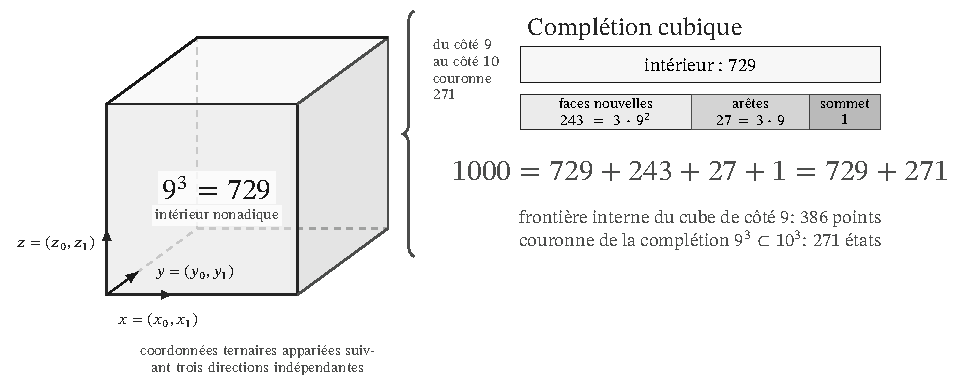
\includegraphics[width=\linewidth]{figures/cubo_emrh.pdf}
\caption{Représentation cubique de l'extension de neuf à dix classes par coordonnée. Les strates \(S_1,S_2,S_3\) placent les incidences ajoutées sur les faces, les arêtes et l'apex ; leurs cardinaux forment la couronne de \(271\) éléments. La frontière de \(386\) éléments appartient au cube initial. La perspective géométrique complète la partition de la figure ~\ref{fig:revision-emrh} ; les séparations graphiques ont une fonction schématique.}
\label{fig:completacion-cubo-recuperado}
\end{figure}


\subsubsection{Conservation de l'unité et compatibilité dimensionnelle}

La normalisation ne se limite pas à diviser une identité isolée. En dimension
\(d\), le produit \(\widehat E^d\) porte la mesure uniforme
\(\mu_d(\{x\})=10^{-d}\). La projection coordonnée
\(p_d:\widehat E^{d+1}\to\widehat E^d\) supprime la dernière coordonnée.

\begin{proposition}[Compatibilité projective des mesures normalisées]
Pour tout \(d\geq1\),
\[
 (p_d)_*\mu_{d+1}=\mu_d,
 \qquad \mu_d(\widehat E^d)=1.
\]
La masse de la strate comportant \(r\) coordonnées supplémentaires est
\(\binom dr9^{d-r}/10^d\), et la somme des masses de toutes les strates
vaut un.
\end{proposition}
\begin{proof}
Chaque point de \(\widehat E^d\) possède dix préimages. Leur masse totale est
\(10\,10^{-(d+1)}=10^{-d}\). L'égalité pour tout sous-ensemble
s'obtient en sommant sur ses points. La formule stratifiée provient
du même dénombrement que \eqref{eq:revision-estratos} ; le binôme
\((9+1)^d\) donne la normalisation totale.
\end{proof}

En dimension trois, retirer l'apex laisse une masse \(999/1000\), et
le restituer ajoute \(1/1000\). Renormaliser avant la restitution
définirait une autre mesure : la distinction est pertinente sur le plan opératoire.
En particulier, conservation de la masse probabiliste, conservation des
registres de transport et dissipation thermodynamique sont des affirmations portant sur
des objets différents. La proposition démontre la première et fournit le
support compatible pour étudier la deuxième ; la troisième requiert une
réalisation dynamique et énergétique spécifiée.

La frontière géométrique interne demeure également distincte.
Sur le représentant cartésien \(\{1,\ldots,9\}^3\), retirer
\(\{2,\ldots,8\}^3\) laisse \(386\) points. Cette frontière appartient au
cube initial, tandis que \(\widehat C\setminus C\) appartient à son
extension. La complétion cubique, le développement positionnel en base mille et
la lecture d'incidence exceptionnelle partagent des données du support ;
leurs applications respectives déterminent l'information issue de ces données qu'utilise
chaque représentation.


\subsection{Incidence cubique et réalisation lorentzienne}

La complétion cubique apporte une relation entre intérieur et frontière.
Sa géométrie peut être développée au moyen de l'incidence des six faces
avec les huit sommets. Étiquetons les faces par \((i,\varepsilon)\),
\(i\in\{1,2,3\}\), \(\varepsilon\in\{+1,-1\}\), et les sommets par
\(\nu\in\{+1,-1\}^3\). La matrice d'incidence est
\[
 M_{(i,\varepsilon),\nu}=\mathbf1_{\{\nu_i=\varepsilon\}}.
\]
Soient \(u=(1,\ldots,1)^{\mathsf T}\in\RR^6\), \(R_F\) l'opposition des faces et \(P_u=uu^{\mathsf T}/6\), \(P_-=(I-R_F)/2\).

\begin{proposition}[Quotient d'incidence de dimension quatre]
Le gramien d'incidence satisfait
\[
 MM^{\mathsf T}=12P_u+4P_-.
\]
Ses valeurs propres \(12,4,0\) ont les multiplicités \(1,3,2\).
En conséquence,
\[
 Q_\square=\RR^6/\ker(MM^{\mathsf T})
 \simeq\RR u\oplus E_-,\qquad E_-=\operatorname{im}P_-.
\]
\end{proposition}
\begin{proof}
Une face contient quatre sommets ; deux faces opposées ont une intersection vide, et deux faces distinctes non opposées partagent deux sommets. La matrice \(12P_u+4P_-\) possède précisément ces entrées. L'espace uniforme est de dimension un ; les différences entre faces opposées engendrent un espace de dimension trois, orthogonal à l'espace uniforme. Son complément est de dimension deux et appartient au noyau.
\end{proof}

La décomposition \(1+3\) procède de l'incidence. Le choix temporel
est déclaré au moyen de la forme bilinéaire
\[
 B_\square([x],[y])=\langle x,(P_--P_u)y\rangle.
\]
Elle est bien définie sur le quotient, car les deux projecteurs annulent le
noyau. Dans la base
\[
 t=[u]/\sqrt6,\qquad
 d_i=[e_{i,+}-e_{i,-}]/\sqrt2,
\]
sa matrice est \(\operatorname{diag}(-1,1,1,1)\). Sont ainsi explicités
le domaine, la décomposition et la convention de signe qui produisent
la réalisation de Minkowski. Le gramien positif détermine le quotient ;
l'affectation temporelle détermine la forme indéfinie sur celui-ci.

L'opérateur
\[
 W_\square=\sqrt6P_u+\sqrt2P_-,\qquad
 W_\square e_{i,\varepsilon}=t+\varepsilon d_i
\]
envoie les six étiquettes de face sur des directions nulles, puisque
\(B_\square(t+\varepsilon d_i,t+\varepsilon d_i)=-1+1=0\).
L'inversion d'une direction et l'opposition des faces disposent ainsi
d'une réalisation géométrique concrète.

\subsubsection{Soudure, inversion et subdivision}

La réalisation cellulaire utilise un transport inversible \(U_m(a)\),
qui conserve la forme lorentzienne, entre les fibres aux extrémités d'une
arête duale orientée \(a\), une étiquette
de face \(\lambda_m(a)\) et une orientation \(\sigma_m(a)\).
Avec \(\ell_m=\ell_0/9^m\), l'application de soudure est
\[
 \beta_m(a)=\ell_m\sigma_m(a)
 W_{\square,s(a)}e_{\lambda_m(a)}.
\]
L'inversion compatible satisfait
\[
 \beta_m(\bar a)=-U_m(a)\beta_m(a).
\]
Identifions les fibres de l'origine à deux niveaux consécutifs au moyen de l'isométrie de raffinement déclarée. Si les neuf sous-segments \(a_1,\ldots,a_9\), de niveau \(m+1\), conservent leur étiquette et leur orientation lorsqu'ils sont transportés vers cette fibre commune, alors
\begin{equation}
 \beta_m(a)=\sum_{j=1}^9
 U_{m+1}(a_1\cdots a_{j-1})^{-1}\beta_{m+1}(a_j).
 \label{eq:soldadura-refinamiento}
\end{equation}
Chaque terme transporté équivaut à \(\ell_m/9\) suivant la même
direction nulle, ce qui démontre l'identité. L'hypothèse de
compatibilité détermine quelles subdivisions réalisent ce raffinement.
L'équation réunit direction, échelle et transport, au lieu de limiter
la correspondance géométrique à un dénombrement des dimensions.

L'orientation et la forme lorentzienne étant également fixées, la dualité de Hodge dans \(\Lambda^2Q_\square^*\) satisfait \(\star^2=-I\). En dimension quatre, le signe est \((-1)^{2(4-2)+1}=-1\). On obtient une structure complexe réelle sur les deux-formes et, après complexification, les sous-espaces propres de valeurs \(+i\) et \(-i\). La réalisation électromagnétique utilisera ce domaine après la construction de la section électronique et la déclaration de son couplage.

\subsection{Compatibilité entre les réductions modulaire et positionnelle}

La base décimale par blocs intervient au moyen d'une division euclidienne
qui conserve simultanément le résidu et le quotient :
\[
 n=1000q+r,\qquad 0\le r<1000.
\]
Puisque \(1000\equiv1\pmod9\) et \(1000\equiv1\pmod3\),
\[
 n\equiv q+r\pmod9,\qquad n\equiv q+r\pmod3.
\]
Par conséquent, la réduction d'un bloc requiert la contribution du
quotient pour restituer la classe de l'entier. Les nombres \(0\) et
\(1000\) ont le même reste modulo \(1000\), mais des classes différentes
modulo \(9\) et modulo \(3\). C'est une raison opératoire de conserver
la mémoire pendant le changement de résolution.

Le raffinement ternaire et la détermination d'un préfixe décimal
peuvent se coordonner au moyen d'un unique résidu entier. Si \(N/3^L\)
est une extrémité de cylindre et \(D/1000^r\) une extrémité décimale, nous définissons
\[
 A=1000^rN-D3^L.
\]
En ajoutant six symboles ternaires, \(N'=729N+\nu\),
\(L'=L+6\), avec \(0\le\nu<729\). Si le préfixe décimal reste
fixe, on obtient
\[
 A'=729A+\nu1000^r.
\]
Si l'on incorpore en outre un bloc décimal \(\delta\), alors \(D'=1000D+\delta\), \(r'=r+1\), et
\begin{equation}
 A'=729000A+\nu1000^{r+1}-729\delta3^L.
 \label{eq:residuo-dos-bases}
\end{equation}
Les deux identités se démontrent en substituant les définitions. La
comparaison des extrémités se réduit ainsi à des opérations entières qui
retiennent la contribution de chaque prolongation. Cette compatibilité
permet de raffiner une région avant d'évaluer sa coordonnée réelle.

% Incorporación al final de extension.tex; no contiene una sección principal.
% Procedencia: RESULTADO_RECUPERADO; explicitación sectorial de las hipótesis.
% Fuentes leídas: monografía Doble proyección holográfica (cantera editorial),
% manuscrito/local/01_tesis_recuperada.tex y
% manuscrito/generated/algebra_holonomica.tex, especialmente §§1--7 y 21.
% Definición rectora de número: manuscrito/flattened/main_autosuficiente.tex,
% secciones que comienzan en líneas 22137 y 23000 de la cantera de 775 páginas.
% No se adopta su presentación global como prueba de todas las flechas TPK.

\subsection{Le nombre comme section compatible et la valeur comme lecture}
\label{hist:seccion}

La distinction entre état et observation permet de préciser quel objet est prolongé lorsque la résolution augmente. À la profondeur \(n\), soit \(X_n\) l'ensemble des états admissibles produits par APP--TRIT--TPK. Leurs données incluent la position, les feuillets somme et produit, les résidus et quotients, le régime, l'orientation, la retenue, la phase, le chemin, la frontière, la mémoire et la survie. Ce ne sont pas des coordonnées indépendantes : les évaluations arithmétiques et les transports précédents imposent leurs relations. Un prolongement conserve ces relations dans chaque antécédent, même s'il ajoute de nouvelles étapes et de nouvelles données de mémoire. Tel est le sens de l'arithmétique des histoires développée de manière autonome dans cet article.

Soient \(r_{m,n}:X_m\to X_n\), pour \(m\geq n\), les restrictions de
profondeur, avec \(r_{n,n}=\operatorname{id}\) et
\(r_{\ell,n}=r_{m,n}\circ r_{\ell,m}\). Chaque restriction conserve le
préfixe et l’information déjà déterminée en lui.

\begin{definition}[Section numérique compatible]
Un nombre HMT est une histoire compatible du système d’états :
\begin{equation}
 x=(x_n)_{n\geq0}\in X_\infty:=\varprojlim_n X_n,
 \qquad r_{m,n}(x_m)=x_n.
 \label{hist:limite-inverso}
\end{equation}
Un lecteur est une opération supplémentaire sur un domaine spécifié de ces
histoires. Un chiffre est une observation finie ; une valeur scalaire est une
évaluation du lecteur. Le couple formé de la section et de son lecteur constitue
une présentation munie d’une lecture, non une redéfinition de l’identité de la section.
\end{definition}

Dans le domaine archimédien \(X_\infty^{\mathrm{Arch}}\), le lecteur associe
à chaque préfixe un cylindre fermé, conserve leur emboîtement et fait tendre
leur diamètre vers zéro. Il détermine ainsi
\begin{equation}
 \operatorname{ev}_{\mathbb R}:X_\infty^{\mathrm{Arch}}\longrightarrow
 \mathbb R,\qquad
 \{\operatorname{ev}_{\mathbb R}(x)\}=\bigcap_n I_n(x).
 \label{hist:evaluacion}
\end{equation}
La construction concrète de ces cylindres et la décision de leurs frontières
sont développées dans la section~\ref{sec:generacion}. La définition
\eqref{hist:limite-inverso} n’affirme pas à elle seule que l’image de
\eqref{hist:evaluacion} soit la droite entière : une affirmation de couverture
requiert son propre théorème. Une égalité de valeurs n’établit pas non plus, sans
résultat d’injectivité, l’égalité de leurs histoires. Cette séparation
permet de parler de précision comme profondeur en conservant la différence
entre l’antécédent arithmétique et sa réalisation scalaire.

\subsection{Composition des histoires et multiplicateur de mémoire}
\label{hist:algebra}

Fixons un secteur d’états à la profondeur \(n\) et une catégorie
\(\mathcal C\) dont les flèches sont leurs histoires admissibles. La composition
s’écrit \(vu=v\circ u\) : on parcourt d’abord \(u\), puis \(v\).
Les pas élémentaires proviennent de la sélection, du transport et de
l’actualisation du TPK. Une fibre tritique locale admet l’écriture
\(\mathbb R[J_x]/(J_x^2+\tau(x)1_x)\), où
\(\tau(x)\in\{+1,0,-1\}\). Le régime et l’orientation appartiennent à
l’état transporté ; une transition entre régimes n’équivaut pas à
l’identification de leurs algèbres quadratiques.

La formulation suivante précise un secteur algébrique de cette composition.
Pour chaque objet \(x\), on se donne une algèbre réelle associative unitaire \(A_x\),
éventuellement non commutative. Pour chaque \(u:x\to y\), on se donne un
homomorphisme unital \(\rho_u:A_x\to A_y\). Nous supposons une action stricte :
\begin{equation}
 \rho_{\operatorname{id}_x}=\operatorname{id}_{A_x},\qquad
 \rho_v\rho_u=\rho_{vu}.
 \label{hist:accion-estricta}
\end{equation}
Pour chaque couple composable \(u:x\to y\), \(v:y\to z\), nous fixons un
multiplicateur central inversible
\(\Omega(v,u)\in Z(A_z)^\times\). On exige la normalisation
\(\Omega(\operatorname{id}_y,u)=\Omega(u,\operatorname{id}_x)=1_y\)
et, pour chaque triplet composable, l’identité
\begin{equation}
 \rho_w\bigl(\Omega(v,u)\bigr)\Omega(w,vu)
   =\Omega(w,v)\Omega(wv,u).
 \label{hist:cociclo}
\end{equation}
Il s’agit d’hypothèses explicites sur les transports et leurs coefficients, non d’une
conséquence du qualificatif holonomique appliqué à la dynamique. Pour appliquer cette présentation
à un secteur TPK, il faut identifier ses \(\rho_u\) et \(\Omega(v,u)\).
Les transitions exprimées par des bimodules exigent la conservation de cette
structure et ne sont pas remplacées par \eqref{hist:accion-estricta}.

L’espace des sommes finies
\[
 \mathcal H(\mathcal C,A,\rho,\Omega)
   =\bigoplus_{u\in\operatorname{Mor}(\mathcal C)} A_{t(u)}T_u
\]
est muni du produit bilinéaire
\begin{equation}
 (aT_v)(bT_u)=a\rho_v(b)\Omega(v,u)T_{vu},
 \label{hist:producto}
\end{equation}
si les flèches sont composables, et de zéro sinon. Ici, \(t(u)\)
désigne l’état terminal. La somme réunit des histoires à coefficients ; le
produit concatène les histoires en conservant le multiplicateur du registre.

\begin{proposition}[Associativité sectorielle à multiplicateur central]
Sous \eqref{hist:accion-estricta} et \eqref{hist:cociclo}, le produit
\eqref{hist:producto} est associatif. Si l’ensemble des objets est fini,
son unité est \(\sum_x1_xT_{\operatorname{id}_x}\).
\end{proposition}
\begin{proof}
Pour \(u:x\to y\), \(v:y\to z\), \(w:z\to t\), soient
\(a\in A_y\), \(b\in A_z\), \(c\in A_t\). Les deux coefficients
de \(T_{wvu}\) sont
\begin{align*}
 ((cT_w)(bT_v))(aT_u):\quad&
 c\rho_w(b)\Omega(w,v)\rho_{wv}(a)\Omega(wv,u),\\
 (cT_w)((bT_v)(aT_u)):\quad&
 c\rho_w(b)\rho_w\rho_v(a)\rho_w(\Omega(v,u))\Omega(w,vu).
\end{align*}
L’action stricte identifie \(\rho_w\rho_v(a)\) à \(\rho_{wv}(a)\).
La centralité de \(\Omega(w,v)\) permet de le déplacer à droite de
ce facteur ; \eqref{hist:cociclo} égalise alors les produits restants.
Les coefficients \(a,b,c\) ne sont pas permutés. Si le triplet n’est pas composable,
les deux parenthésages sont nuls du fait de leurs états initiaux et terminaux.
La bilinéarité achève la preuve. Les identités locales et la
normalisation de \(\Omega\) vérifient l’unité indiquée.
\end{proof}

La retenue du calendrier fournit un exemple effectif. Dans la catégorie
à un objet et de flèches \(C_9\), prenons pour coefficients
\(A=\mathbb R[z,z^{-1}]\), l’action identité et
\[
 \Omega(b,a)=z^{c_0(a,b)},\qquad
 c_0(a,b)=\left\lfloor\frac{a+b}{9}\right\rfloor,
 \quad 0\leq a,b<9.
\]
Les deux sommes de retenues d’un triplet sont
\(\lfloor(a+b+c)/9\rfloor\) ; \eqref{hist:cociclo}
est donc satisfaite. La variable formelle \(z\) enregistre le tour sans
lui attribuer de valeur numérique. Imposer ensuite \(z^{12}=1\) restitue le
registre dodécaphasique du calendrier \eqref{eq:extension108} ; conserver
\(z\) sans cette relation distingue les tours successifs. L’exemple réalise
la mémoire de ce calendrier, sans l’identifier à la totalité de la
mémoire TPK.

\subsection{Double variance du raffinement et conservation de l’unité}
\label{hist:doble-varianza}

La restriction des états prolonge les observables en sens contraire.
Considérons les algèbres de fonctions, munies du produit ponctuel,
\(D_n=\operatorname{Fun}(X_n,\mathbb R)\). La précomposition définit
\begin{equation}
 r_{m,n}^*:D_n\longrightarrow D_m,
 \qquad r_{m,n}^*f=f\circ r_{m,n}.
 \label{hist:precomposicion}
\end{equation}
Ce sont des morphismes unitaux ; ils sont également injectifs lorsque les restrictions
correspondantes sont surjectives. La limite inductive
\(D_{\mathrm{cyl}}=\varinjlim_n(D_n,r_{n+1,n}^*)\) réunit les
observations de profondeur finie. Cette algèbre n’est pas identifiée ici
à l’algèbre entière des routes : prolonger les opérateurs de transport exige
également leurs compatibilités avec le raffinement.

\begin{lemma}[Unité et naturalité de l’évaluation]
Si \(e_x\) est l’indicatrice de \(x\in X_n\), on a
\begin{equation}
 r_{m,n}^*e_x=\sum_{y:\,r_{m,n}(y)=x}e_y,
 \qquad r_{m,n}^*1_n=1_m,
 \label{hist:unidad}
\end{equation}
et, pour tous \(f\in D_n\), \(y\in X_m\),
\[
 \langle r_{m,n}^*f,y\rangle=\langle f,r_{m,n}y\rangle.
\]
Chaque section \(x\in X_\infty\) détermine une évaluation bien définie
\(D_{\mathrm{cyl}}\to\mathbb R\), donnée par \([f]\mapsto f(x_n)\)
pour \(f\in D_n\).
\end{lemma}
\begin{proof}
Les fibres de \(r_{m,n}\) forment une partition de \(X_m\). Leurs
indicatrices sont orthogonales et de somme \(1_m\), ce qui démontre
\eqref{hist:unidad}. La naturalité est la définition de la précomposition.
Enfin, \((r_{m,n}^*f)(x_m)=f(x_n)\), de sorte que deux représentants
compatibles donnent la même évaluation dans la limite inductive.
\end{proof}

L’unité globale est la fonction constante un sur toutes les possibilités ;
la section individuelle sélectionne une histoire compatible. Conserver la
première ne signifie pas immobiliser la seconde. Le raffinement peut augmenter
le nombre d’extensions et la profondeur de chaque histoire en maintenant
l’unité et toutes les évaluations de ses antécédents.

\subsection{Retour de phase, représentation de Weyl et deux lectures}
\label{hist:puente-lecturas}

La loi \eqref{eq:holonomia-memoria} acquiert une réalisation opératorielle
dans la suspension bilatérale qui sera construite dans la
section~\ref{sec:generacion}. Dans celle-ci, \(T\) est l’avancement d’un pas,
\(V_9\) observe la phase nonadique, \(W_\delta\) la phase de rotation et
\(D_M\) le degré de mémoire. En écrivant
\(\widehat\Gamma_9=T^9\) pour le tour dans cette représentation,
les relations de Weyl \eqref{eq:weyl-relojes} impliquent, sur les vecteurs
de support fini,
\begin{equation}
 \begin{aligned}
 V_9\widehat\Gamma_9&=\widehat\Gamma_9V_9,\qquad
 W_\delta\widehat\Gamma_9=e^{2\pi i9\delta}
     \widehat\Gamma_9W_\delta,\\
 [D_M,\widehat\Gamma_9]&=\widehat\Gamma_9.
 \end{aligned}
 \label{hist:tres-retornos}
\end{equation}
La première égalité découle de \(\zeta_9^9=1\) ; la deuxième, de neuf
applications de la covariance de \(W_\delta\) ; la troisième exprime
l’incrément unitaire de mémoire. La phase finie revient, tandis que la
rotation irrationnelle et la mémoire distinguent l’état suivant. Les
caractères et le paramètre \(\delta\) sont réalisés ultérieurement à partir de la
construction numérique spécifiée dans cette section : ils ne sélectionnent pas rétrospectivement
les conditions initiales. Cette représentation décrit les observables et les translations de
la suspension ; elle ne remplace ni toutes les coordonnées ni tous les opérateurs
du TPK.

La double lecture prolonge la même distinction entre histoire et observable.
Dans son domaine archimédien, on applique \eqref{hist:evaluacion} ; dans le
domaine incidenciel enrichi, les applications \(Q_n\) de la
section~\ref{exc:doble-lectura} conservent les mots et les repères de
frontière. L’égalité qui y est démontrée
\(r_{n,m}Q_n=Q_mp_{n,m}\) détermine son prolongement \(Q_\infty\).
Sur le domaine commun des deux lectures, on peut considérer conjointement
\(\operatorname{ev}_{\mathbb R}(x)\) et \(Q_\infty(x)\) : la
première retient la valeur ; la seconde, l’incidence transportée que son
codomaine conserve. La section précède les deux. Cette articulation permet
de passer de l’arithmétique des histoires aux constantes et à la lecture
exceptionnelle sans transformer leurs réalisations en nouvelles données initiales.

